This chapter presents all the experiments performed about matrix multiplication acceleration and GNN acceleration along with the achieved results.

All the CPU experiments have been conducted using an Intel Core i9, with 8 cores and a frequency of 2,3 GHz.
On the other hand, the synthesis experiments targeted an AMD Virtex UltraScale+ (Alveo U280) FPGA\@.
The whole experimental phase focused on the computational time of the accelerators, assuming that all data are loaded from BRAMs, requiring two cycles to read data and one cycle to store data.


\section{Model analysis and profiling}
\label{sec:model-analysis}%

\begin{table}[b]
\centering
    \begin{tabular}{|p{6em} c c c c|}
    \hline
%    \rowcolor{black!40}
    \textbf{Name} & \textbf{Self CPU \%} & \textbf{Self CPU} & \textbf{CPU total \%} & \textbf{CPU total} \T\B \\
    \hline \hline
    \textbf{aten::mm} & 50,25\% & 1,012$ms$ & 89,72\% & 1,807$ms$ \T\B\\
    \hline
    \textbf{aten::addmm} & 36,30\% & 731,0$\mu s$ & 37,04\% & 746,0$\mu s$ \T\B\\
    \hline
    \textbf{aten::add} & 4,67\% & 94,0$\mu s$ & 4,67\% & 94,0$\mu s$ \T\B\\
    \hline
    %\textbf{aten::\_log\_softmax} & 2,98\% & 60,0us & 2,98\% & 60,0us \T\B\\
    %\hline
    \end{tabular}
    \\[10pt]
    \caption[Excerpt of GCN model inference profiling result]{Excerpt of GCN model inference profiling result. \lstinline{aten::mm}=matrix multiplication; \lstinline{aten::add}=matrix sum; \lstinline{aten::addmm}=matrix multiplication plus matrix sum.}
    \label{tab:gcn_profiling}
\end{table}

As already anticipated in Section~\ref{sec:toolchain-pytorch}, the GCN model is implemented in PyTorch, and it is characterized by two convolutional layers, a ReLU and a dropout functions.
The forward function of each layer contains two matrix multiplications, and one of the two is a sparse multiplication.

The first step to understand how to accelerate the PyTorch GCN model was to analyze and profile it.
Table~\ref{tab:gcn_profiling} shows the results extracted from a run of the PyTorch profiler, which measures the execution times of operations from the ATen~\cite{aten} tensor library that serves as the foundation for most Python and C++ interfaces within PyTorch.
ATen provides a central Tensor class, on which many hundreds of operations are defined.
The majority of these operations have both CPU and GPU implementations, to which the Tensor class dynamically dispatches based on its type.

Among the profiled operations, \lstinline{aten::mm} performs a multiplication between two tensors, \lstinline{aten::addmm} performs a multiplication between two tensors and then another tensor is added to the result and finally \lstinline{aten::add} returns the sum of two tensors provided as input.
The distinction between \textit{self CPU time} and \textit{total CPU time} lies in the fact that self CPU time does not contain the time spent in child operator calls, whereas total CPU time contains it, considering that operators can invoke other operators.
It is clear that the bottleneck and the most time-consuming operation is the matrix multiplication.
In particular, more than 50\% of the self CPU time is used by matrix multiplication, while, considering the child operator calls, this percentage represents nearly the 90\%.
This result clearly justifies a special focus on matrix multiplication acceleration.

\section{Matrix multiplication acceleration}
\label{sec:matmul-acceleration}%

\subsection{PyTorch matrix multiplication benchmark}
\label{subsec:pytorch-matmul-bench}%

PyTorch provides different matrix representations and different matrix multiplication functions.
The one considered in this subsection are \textit{torch.mm} and \textit{torch.spmm}.
The former function multiplies two dense matrices, but it also supports COO and CSR representation.
The latter, instead, is typically used for sparse matrix multiplications, in which one of the two matrices, or both, are saved using sparse representations.

Table~\ref{tab:torch-mm-benchmark} represents a benchmark for the dense matrix multiplication between a first matrix of size $15 \times 15$ and a second matrix of size $15 \times 16$, both composed by float32 elements.
The chosen sizes for input matrices are not arbitrary; they have been specifically selected due to their extensive use in the following experiments, requiring an accurate benchmark for comparison purposes.
In particular, the table shows five different runs, each composed by a different number of executions.
Then, the final time is computed as the average of the five different runs.
Additionally, this average has been computed five times using increasing number of executions.
The results shows that the variance of the runs of the last experiments is lower than the others, fixing to ten millions a sufficient number of executions for good accuracy and stability.

As expected, given the globally high amount of executions, the five average execution times are similar between them, and the variance decreases as the number of executions increases.
In conclusion, the time needed by a dense matrix multiplication between two matrices of the given size can be considered equal to 1.608$\mu s$.
%The Python timing corresponding to the accelerated matrix multiplication for each experiment has been computed using an average of ten million executions.

Since the GCN model uses both dense and sparse matrix multiplication functions, Table~\ref{tab:torch-matmul-comparison} shows the times needed by both functions according to different representations of the two input matrices A and B\@.
Different experiments have been performed using randomly generated input matrices; they are composed by float32 elements and different input sized and levels of sparsity have been analyzed.

\begin{table}[t]
\centering
    \resizebox{\textwidth}{!}{
    \begin{tabular}{|p{6em} c c c c c c|}
    \hline
    \thead{Executions} & \thead{Run1} & \thead{Run2} & \thead{Run3} & \thead{Run4} & \thead{Run5} & \thead{\makecell{Avg. time}} \T\B \\
    \hline \hline
    \makecell{2E06} & 1.587E-06 & 1.568E-06 & 1.567E-06 & 1.594E-06 & 1.572E-06 & 1.578E-06 \T\B\\
    \hline
    \makecell{4E06} & 1.598E-06 & 1.585E-06 & 1.592E-06 & 1.602E-06 & 1.599E-06 & 1.595E-06 \T\B\\
    \hline
    \makecell{6E06} & 1.601E-06 & 1.614E-06 & 1.603E-06 & 1.603E-06 & 1.608E-06 & 1.606E-06 \T\B\\
    \hline
    \makecell{8E06} & 1.608E-06 & 1.607E-06 & 1.600E-06 & 1.614E-06 & 1.617E-06 & 1.609E-06 \T\B\\
    \hline
    \makecell{10E06} & 1.614E-06 & 1.603E-06 & 1.603E-06 & 1.613E-06 & 1.607E-06 & 1.608E-06 \T\B\\
    \hline
    \end{tabular}
    }
    \\[10pt]
    \caption[Benchmark of \textit{torch.mm} PyTorch function]{Benchmark of \textit{torch.mm} PyTorch function. Five runs using different number of executions and their average, execution times reported in seconds.}
    \label{tab:torch-mm-benchmark}
\end{table}

\begin{table}[t]
\centering
    \resizebox{\textwidth}{!}{
    \begin{tabular}{|p{6em} c c c c c c c c|}
    \hline
    \textbf{Function} & \textbf{Sizes} & \textbf{Sparsity} & \textbf{Runs} & \textbf{Dense$\times$Dense} & \textbf{COO$\times$Dense} & \textbf{COO$\times$COO} & \textbf{CSR$\times$Dense} & \textbf{CSR$\times$CSR} \T\B \\
    \hline \hline
    \textbf{torch.mm} & 15$\times$15, 15$\times$16 & 0.9 & 10E06 & \textbf{1.599E-06} & 2.844E-06 & 1.658E-05 & 1.058E-05 & 8.632E-05 \T\B\\
    \hline
    \textbf{torch.spmm} & 15$\times$15, 15$\times$16 & 0.9 & 10E06 & 1.934E-06 & 3.385E-06 & 1.750E-05 & 1.183E-05 & 1.746E-05 \T\B\\
    \hline \hline
    \textbf{torch.mm} & 150$\times$150, 150$\times$16 & 0.9 & 1E06 & \textbf{5.220E-06} & 4.303E-05 & 1.058E-04 & 1.384E-05 & 1.393E-04 \T\B\\
    \hline
    \textbf{torch.spmm} & 150$\times$150, 150$\times$16 & 0.9 & 1E06 & 6.593E-06 & 4.659E-05 & 1.143E-04 & 1.461E-05 & 1.090E-04 \T\B\\
    \hline \hline
    \textbf{torch.mm} & 150$\times$150, 150$\times$16 & 0.99 & 1E06 & 5.752E-06 & 7.039E-06 & 1.887E-05 & 1.256E-05 & 8.730E-05 \T\B\\
    \hline
    \textbf{torch.spmm} & 150$\times$150, 150$\times$16 & 0.99 & 1E06 & \textbf{4.678E-06} & 7.797E-06 & 1.883E-05 & 1.214E-05 & 1.847E-05 \T\B\\
    \hline \hline
    \textbf{torch.mm} & 2708$\times$2708, 2708$\times$16 & 0.999 & 100E03 & 1.288E-03 & 2.030E-04 & 1.325E-04 & \textbf{3.377E-05} & 1.073E-04 \T\B\\
    \hline
    \textbf{torch.spmm} & 2708$\times$2708, 2708$\times$16 & 0.999 & 100E03 & 1.255E-03  & 2.012E-04 & 1.316E-04 & 3.661E-05 & 1.186E-04 \T\B\\
    \hline
    \end{tabular}}
    \\[10pt]
    \caption[Comparison between dense and sparse PyTorch matmul functions]{Comparison between dense and sparse PyTorch matmul functions, computed as average of multiple runs. Execution times reported in seconds.}
    \label{tab:torch-matmul-comparison}
\end{table}

%\begin{figure}[t]
%    \centering
%    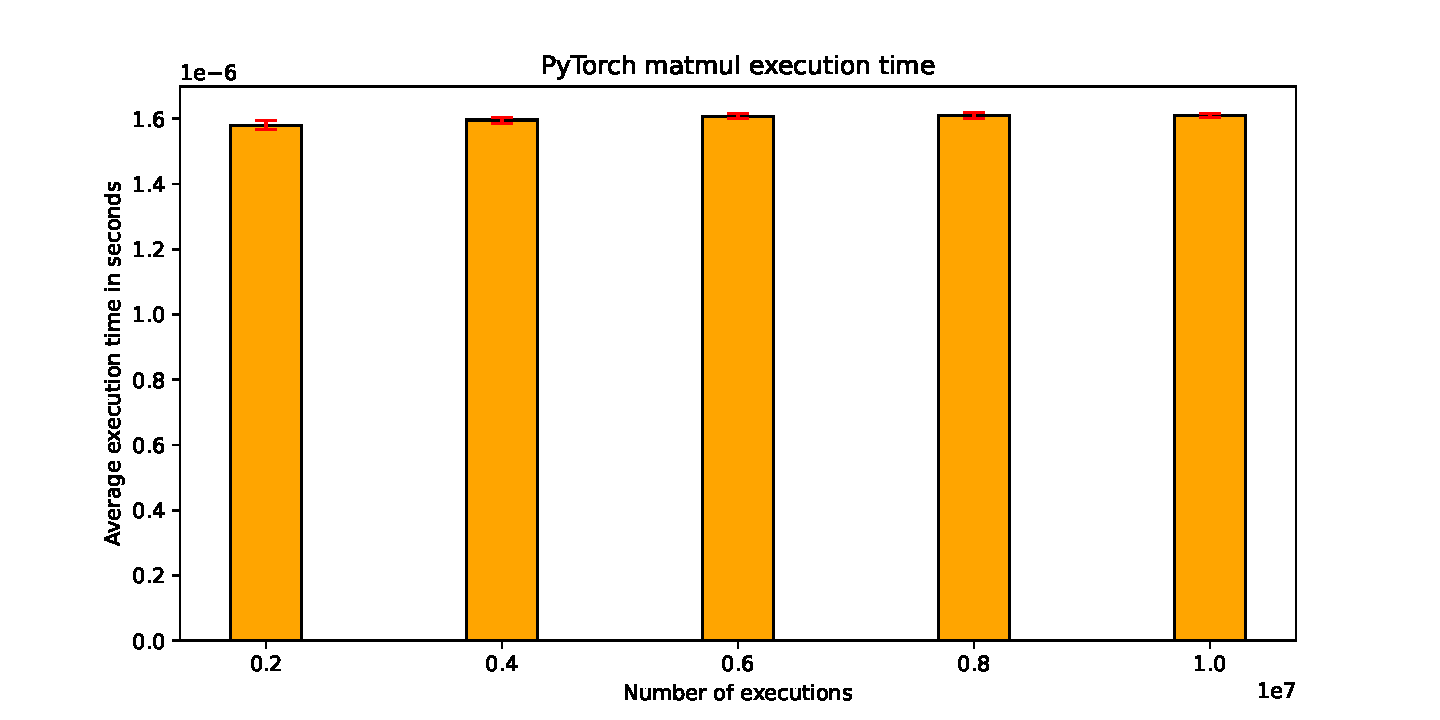
\includegraphics[height=0.4\textwidth]{Images/torch-mm_benchmark}
%    \caption{Benchmark of \textit{torch.mm} PyTorch function}
%    \label{fig:torch-mm_benchmark}
%\end{figure}

It is clear that sparse matrix multiplication, both with dense and sparse matrix representations, does not increase performance on CPU architecture when the size of input matrices is small.
The disadvantage of using sparse matrix multiplication on CPU becomes more evident as the size of the input matrices increases but the level of sparsity remains constant.
However, when the size of input matrices increases considerably and the level of sparsity is very high, using sparse representations, in particular CSR, can bring a significant advantage.

Even if the following experiments do not take advantage of sparse matrix computations, the utilization of custom optimizations for the analyzed GCN has enabled the acceleration of inference, balancing the absence of sparse matrix computations.

\subsection{FPGA-accelerated matrix multiplication}
\label{subsec:optimization-comparison}%

Before applying any optimization, it is necessary to understand the difference between PyTorch matrix multiplication operation and the baseline accelerator.
To obtain the baseline matmul accelerator, the process began with following the initial steps of the toolchain described in Chapter~\ref{ch:chapter_five} using the GCN model.
After having made the model compatible with TorchScript, its linalg representation has been obtained through Torch-MLIR compilation.
Subsequently, only the matmul code of the generated MLIR representation has been outlined through SODA annotations instead of selecting the whole GCN model.
After lowering and optimizing the resulting kernel, its LLVM IR has been synthesized with PandA-Bambu, including the \lstinline{-fno-unroll-loops} flag, options to request two memory channels, and the \lstinline{ALL_BRAM} option requesting that all data is stored in on-chip block RAMs.
Figure~\ref{fig:pytorch-accelerator-comparison} shows the result of this analysis, which reveal the fact that the cycle counts required by the accelerator for each experiment align perfectly with the anticipated expectations outlined in Section~\ref{sec:matmul-algo}.
Specifically, dividing the cycle count of the first experiment of the table and the final one by the total count of loop iterations effectively confirms a consistent result of approximately 7 in both instances, corresponding to the second part of Equation~\ref{eq:number-cycles}.

The PyTorch times have been recorded by averaging five measurements each of ten millions executions.
The baseline accelerator is much faster than PyTorch when matrices are relatively small.
The reason behind this behavior may lie in the fact that the generated accelerator simplifies data loading by assuming that all data is available in BRAM. By default, the system uses two channels and stores all memory objects in BRAMs.
However, an alternative approach, explored in this thesis, to further optimize the matmul accelerator, involves employing a greater number of memory channels while utilizing external memory.
The advantage of the accelerator in terms of performance decreases as the size of the input matrices increase, until reaching a point in which the accelerator becomes slower than PyTorch solution.

%\begin{table}[t]
%\centering
%    \begin{tabular}{|p{9em} c c c c  |}
%    \hline
%    \textbf{Input sizes} & \textbf{Torch.mm (s)} & \textbf{Runtime (s)} & \textbf{Cycles} & \textbf{SpeedUp} \T\B \\
%    \hline \hline
%    \textbf{15$\times$15, 15$\times$16} & 1.60E-06  & 96.49E-09 & 25,697 & 16.58 \T\B\\
%    \hline
%    \textbf{30$\times$30, 30$\times$16} & 1.73E-06  & 351.18E-09 & 101,792 & 4.92 \T\B\\
%    \hline
%    \textbf{60$\times$60, 60$\times$16} & 2.48E-06  & 1.46E-06 & 405,182 & 1.69 \T\B\\
%    \hline
%    \textbf{90$\times$90, 90$\times$16} & 4.55E-06  & 3.15E-06 & 910,172 & 1.44 \T\B\\
%    \hline
%    \textbf{120$\times$120, 120$\times$16} & 4.79E-06  & 5.62E-06 & 1,616,762 & 0.85 \T\B\\
%    \hline
%    \textbf{150$\times$150, 150$\times$16} & 5.16E-06  & 9.07E-06 & 2,524,952 & 0.56 \T\B\\
%    \hline
%    \end{tabular}
%    \\[10pt]
%    \caption{Comparison between dense and sparse PyTorch matmul functions}
%    \label{tab:pytorch-accelerator-comparison}
%\end{table}

\begin{figure}[t]
    \centering
    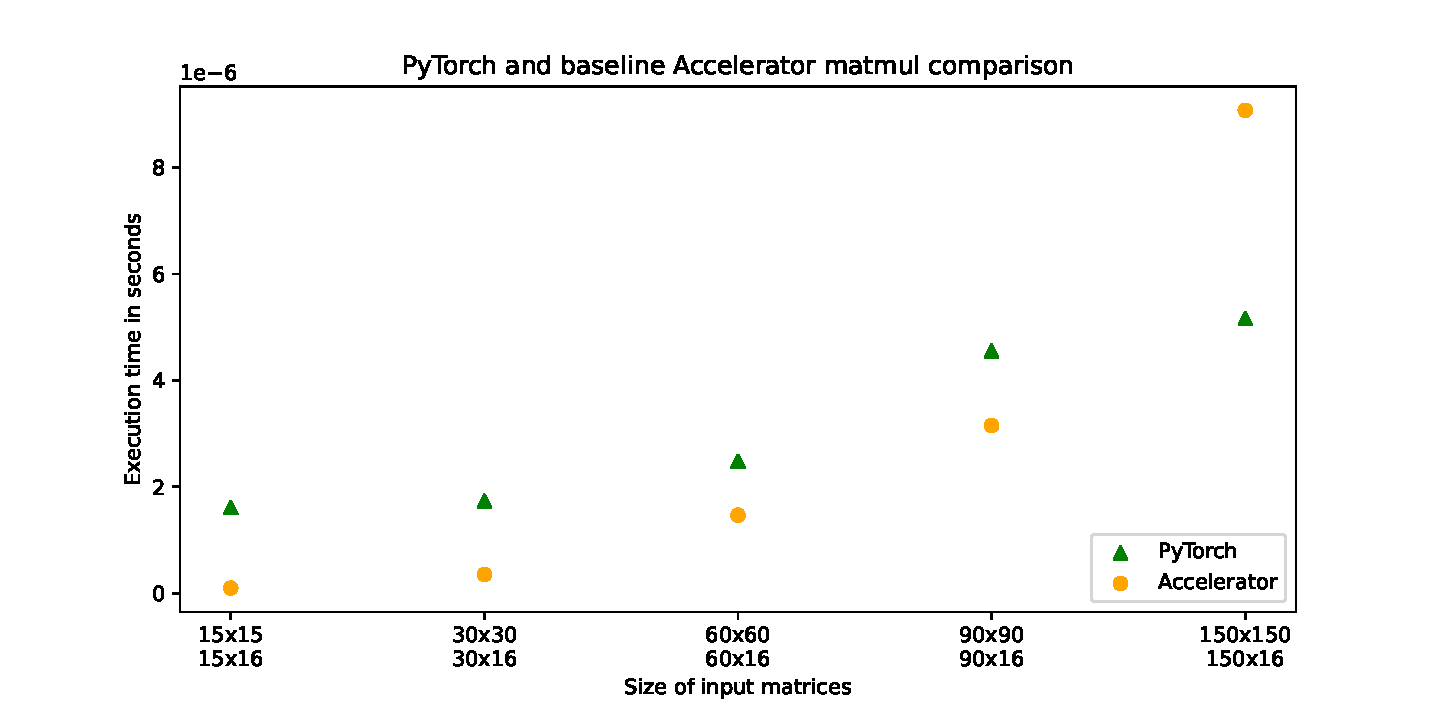
\includegraphics[height=0.4\textwidth]{Images/matmul_comparison}
    \caption{Performance comparison between PyTorch matmul function and accelerator}
    \label{fig:pytorch-accelerator-comparison}
\end{figure}

Another possible factor may be that PyTorch times have been recorded using all the eight available threads on the machine.
So, it is expected that the \lstinline{torch.mm} function exploits more parallelism with respect to the accelerator, and this advantage is more evident when the potential level of parallelism increases.
For this reason, the optimizations discussed in Section~\ref{subsec:toolchain-soda_opt} and in Section~\ref{subsec:toolchain-panda_bambu} need to be applied to exploit more parallelism.

SODA-OPT, as introduced in Subsection~\ref{subsec:toolchain-soda_opt}, offers the possibility to make different types of unrolling, among which the full unroll which completely unroll the innermost loop, and the partial unroll up to an arbitrary factor.
Moreover, PandA-Bambu introduces several optimization options, one of which, as already anticipated above, involves expanding the number of memory channels in use by exploiting an external memory instead of a BRAM\@.

The combination of loop unrolling and multiple memory channels offers both advantages and disadvantages, resulting in a trade-off.
Loop unrolling enhances parallelization, thereby reducing computational time.
However, especially when utilizing more than two memory channels, it increases the number of parallel processing elements, leading to a larger area footprint.
External memory allows for up to 32 memory channels, enabling the simultaneous loading of 32 variables; nonetheless, accessing data from external memory may require more load cycles compared to accessing internal memory, depending by the access time of DDRs.
During the conducted experiments, both internal and external memory requires two cycles for data loading and one cycle for data storage.
However, when not utilizing BRAM, which is pipelined with an initiation interval of one, a factor taken into consideration during scheduling, it leads to an increase in the number of cycles for the accelerator, resulting from the loss of pipelining.

\begin{figure}[t]
    \centering
    \subfloat[Input matrices $15\times15$, $15\times16$\label{fig:matmul-optimization-comparison15}]{
        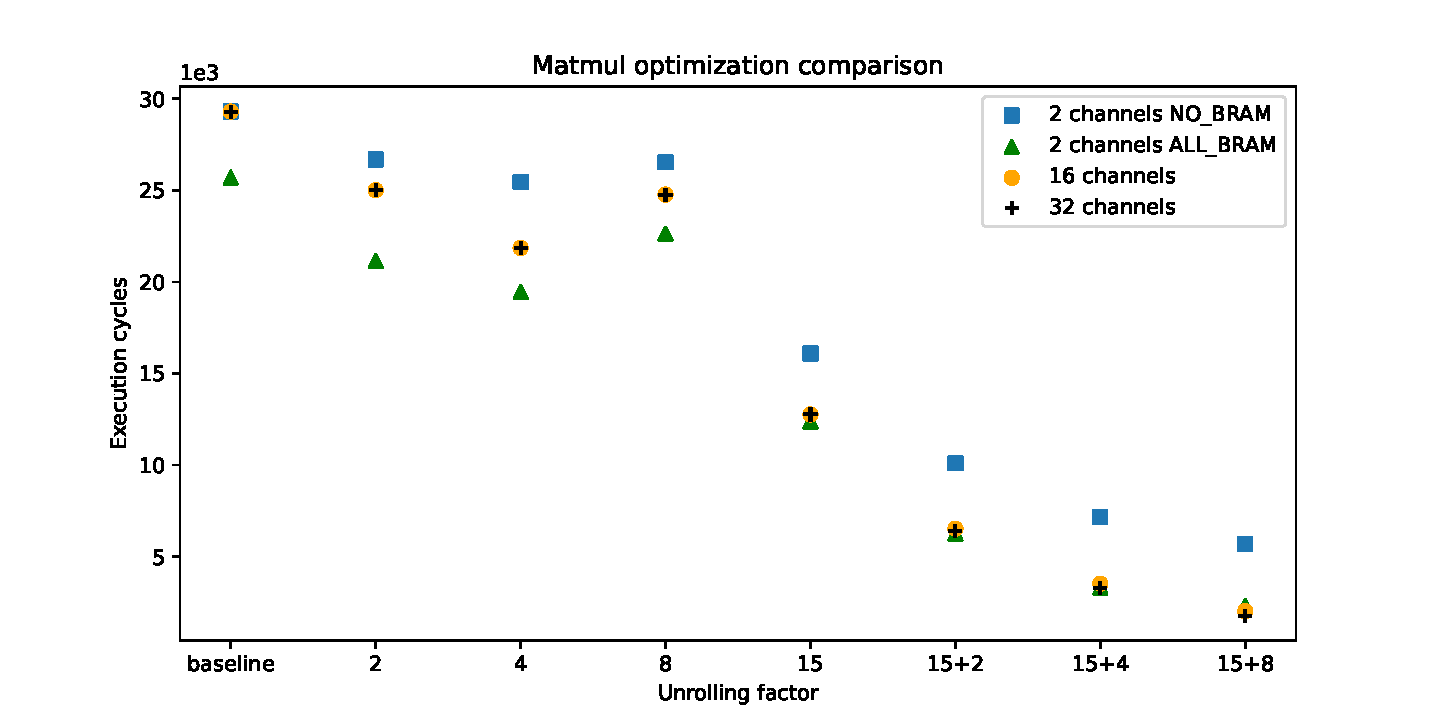
\includegraphics[height=0.4\textwidth]{Images/matmul_comparison15}
    }
    %\quad
    \hspace{0.15\textwidth}
    \subfloat[Input matrices $30\times30$, $30\times16$\label{fig:matmul-optimization-comparison30}]{
        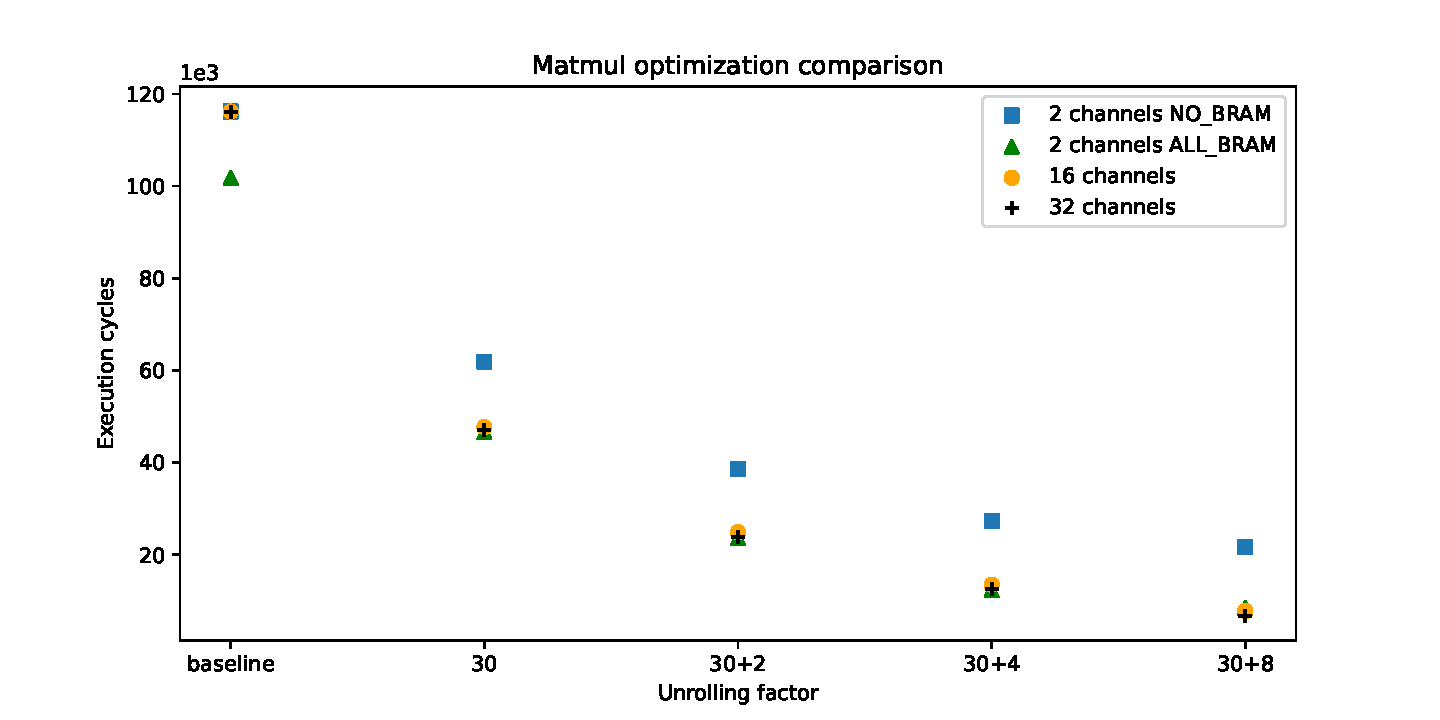
\includegraphics[height=0.4\textwidth]{Images/matmul_comparison30}
    }
    \caption{Matrix multiplication optimization comparison}
    \label{fig:matmul-optimization-comparison}
\end{figure}

Figure~\ref{fig:matmul-optimization-comparison} show the performance of two matrix multiplication accelerators operating on different sizes of the input matrices.
Figure~\ref{fig:matmul-optimization-comparison15} show results of a multiplication between two matrices of size $15\times15$ and $15\times16$, while Figure~\ref{fig:matmul-optimization-comparison30} shows results of a multiplication between two matrices of size $30\times30$ and $30\times15$.
In both figures, on the x-axis there is the unrolling factor used and on the y-axis the resulting number of cycles.
The baseline computation does not use unrolling, instead when there are two factors it means that the first one can be considered as a full unroll of the innermost cycle, while the second one is the unrolling factor applied to the original second innermost cycle.

In both cases, when the parallelization is not high, thus the unrolling factor is small, using two channels and storing all memory objects in BRAMs is the best option since a minor number of cycles is required to perform the computation.
Using 16 channels seems to be similar to using 32 channels, but when parallelization is high the latter option uses fewer cycles.
As expected, the findings indicate that opting for two channels with external memory is the least favorable choice.
This is primarily because employing external memory becomes advantageous when a large volume of data can be simultaneously loaded and stored to offset the additional cycles required for external memory access.

The best trade-off is achieved using an unrolling factor for which the number of cycles needed by the accelerator with 32 memory channels is lower than the number of cycles needed by the accelerator with 2 memory channels.
In the first case, in Figure~\ref{fig:matmul-optimization-comparison15}, this objective is achieved with two unrolling factors of 15 and 8, while in the second case is achieved with unrolling factors of 30 and 8.

These results can be used to set a heuristic useful to identify the number of parallel unrolled loop iterations that makes the use of 32 channels with external memory preferable to the use of 2 channels with BRAM:

\begin{equation}
    \label{eq:factor-relation}
        i \cdot j \cdot k \geq 2 \cdot \sqrt {M \cdot N \cdot R}
\end{equation}

where $M$, $N$ and $R$ are the sizes of the three nested loops, as defined in Algorithm~\ref{alg:var}, and $i$, $j$ and $k$ are their respective loop unrolling factors, following the rule $j \neq 1 \iff i=M \land k \neq 1 \iff j=N$.

Equation~\ref{eq:factor-relation} captures the parameters leading to the two results.
In fact, using 15 and 8 as unrolling factors means having $15 \cdot 8 = 120$ parallel loop iterations.
Instead, using 30 and 8 as unrolling factors means having $30 \cdot 8 = 240$ parallel loop iterations.
Additionally, the total amount of possible parallel loop iterations in a matrix multiplication between two matrices of sizes $15\times15$ and $15\times16$ is equal to $15 \cdot 16 \cdot 15 = 3,600$.
Meanwhile, the total amount of possible parallel loop iterations in a matrix multiplication between two matrices of sizes $30\times30$ and $30\times16$ is $30 \cdot 16 \cdot 30 = 14,400$.
Even if the two number of parallel loop iterations representing the changing point of the trade-off are different, 120 and 240, they are related by Equation~\ref{eq:factor-relation}.

Equation~\ref{eq:factor-relation} should not be taken as an infallible rule, but it can be used as a discriminant to decide when to use 32 memory channels instead of two.
In conclusion, the generalized rule is that the number of parallel unrolled loop iterations that justify the use of 32 channels is given by Equation~\ref{eq:factor-relation}.

\section{GCN accelerator evaluation}
\label{sec:gcn_accelerator_evaluation}%

\begin{table}[t]
\centering
    \begin{tabular}{|p{4em} c c c c c|}
    \hline
    \textbf{Name} & \textbf{Nodes} & \textbf{Words} & \textbf{Links} & \textbf{Task} & \textbf{Classes} \T\B \\
    \hline \hline
    \textbf{Cora} & 2708  & 1433 & 5429 & Multiclass classification & 7 \T\B\\
    \hline
    \textbf{Cora15} & 15  & 15 & 3 & Multiclass classification & 7 \T\B\\
    \hline
    \textbf{Cora30} & 30  & 30 & 4 & Multiclass classification & 7 \T\B\\
    \hline
    \textbf{Cora60} & 60  & 60 & 8 & Multiclass classification & 7 \T\B\\
    \hline
    \textbf{Cora90} & 90  & 90 & 18 & Multiclass classification & 7 \T\B\\
    \hline
    \textbf{Cora120} & 120  & 120 & 22 & Multiclass classification & 7 \T\B\\
    \hline
    \textbf{Cora150} & 150  & 150 & 37 & Multiclass classification & 7 \T\B\\
    \hline
    \end{tabular}
    \\[10pt]
    \caption{Cora sub-dataset used for GCN infernce}
    \label{tab:dataset-definition}
\end{table}

%\begin{table}[t]
%\centering
%    \begin{tabular}{|p{4em} c c c c|}
%    \hline
%    \thead{Dataset} & \thead{CPU PyTorch(s)} & \thead{Optimizations} & \thead{Runtime(s)} & \thead{SpeedUp} \T\B \\
%    \hline \hline
%    \makecell{Cora15} & 59.25E-06 & \makecell{Full Unroll} & 523.24E-09 & 113.23 \T\B\\
%    \hline
%    \makecell{Cora30} & 66.42E-06 & \makecell{Full Unroll} & 1.79E-06 & 37.10 \T\B\\
%    \hline
%    \makecell{Cora60} & 69.75E-06 & \makecell{Full Unroll} & 7.13E-06 & 9.78 \T\B\\
%    \hline
%    \makecell{Cora90} & 88.88E-06 & \makecell{Full Unroll} & 14.90E-06 & 5.96 \T\B\\
%    \hline
%    \makecell{Cora120} & 98.32E-06 & \makecell{Full Unroll} & 29.64E-06 & 3.31 \T\B\\
%    \hline
%    \makecell{Cora150} & 115.03E-06 & \makecell{Full Unroll} & 41.12E-06 & 2.79 \T\B\\
%    \hline
%    \end{tabular}
%    \\[10pt]
%    \caption{GCN inference time comparison}
%    \label{tab:GCN-inference-pytorch-accelerator-comparison}
%\end{table}

\begin{figure}[t!]
    \centering
    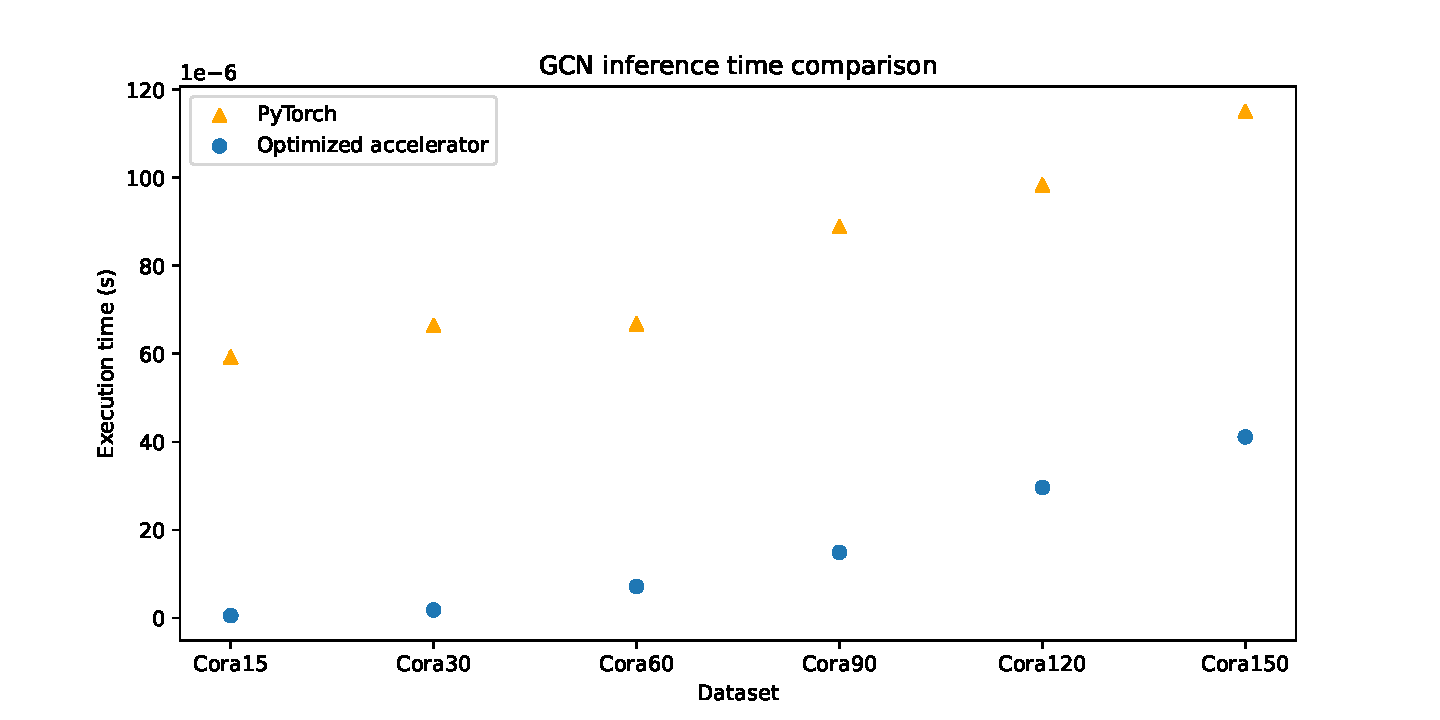
\includegraphics[height=0.4\textwidth]{Images/gcn_forward_comparison}
    \caption{GCN inference PyTorch-Accelerator comparison}
    \label{fig:gcn-inference-comparison}
\end{figure}

In this Subsection, the toolchain and the proposed optimizations are applied to the GCN model.
Figure~\ref{fig:gcn-inference-comparison} shows the result of a comparative analysis between the PyTorch CPU time and the optimized FPGA accelerator time to perform GCN inference.
All the experiments have been performed using a subset of the Cora dataset introduced in Subsection~\ref{subsec:toolchain-inputs}, as detailed in Table~\ref{tab:dataset-definition}.
The PyTorch times have been acquired averaging one million of execution time measurements using the PyTorch built-in benchmark API\@.

Both accelerators have been obtained from the same PyTorch model, which has been lowered using Torch-MLIR\@.
After obtaining the MLIR representation and outlining the entire forward function, the model has been synthesized using SODA-OPT and PandA-Bambu, employing both baseline and optimized configurations.
Figure~\ref{fig:gcn-inference-cycles-comparison} and Table~\ref{tab:GCN-inference-accelerators-comparison} show how the accelerator has been affected by the unrolling technique with respect to the baseline performance.
The optimized settings uses two channels and one full unrolling of the innermost loop, and it obviously requires more area than the baseline accelerator, but it is computationally faster; being matrix multiplication the most time-consuming operation of the GCN, thanks to loop unrolling technique, the speedup increases as the size of the dataset increases as the number of nodes in the graph affects the size of the loop.
The used optimized setting with two channels and BRAM has been preferred to the alternative considered setting with thirty-two channels and two external memory, because it already achieves high speedup without increasing too much area requirements, representing the best trade-off for the considered experiment.

\begin{table}[t]
\centering
    \resizebox{\textwidth}{!}{
    \begin{tabular}{|p{4em} c c c c c c c c c|}
    \hline
    \thead{Dataset} & \thead{Optimizations} & \thead{Cycles} & \thead{Slices} & \thead{Luts} & \thead{Registers} & \thead{DSPs} & \thead{BRAMs} & \thead{Frequency(MHz)} & \thead{SpeedUp} \T\B \\
    \hline \hline
    \makecell{Cora15} & \makecell{Baseline} & 115,852 & 8,307 & 32,927 & 32,195 & 16 & 256 & 147.77 & - \T\B\\
    \hline
    \makecell{Cora15} & \makecell{Full Unroll} & 93,705 & 8,338 & 36,265 & 35,164 & 44 & 256 & 179.08 & 1.23 \T\B\\
    \hline \hline
    \makecell{Cora30} & \makecell{Baseline} & 385,874 & 7,457 & 30,379 & 26,925 & 16 & 256 & 158.25 & - \T\B\\
    \hline
    \makecell{Cora30} & \makecell{Full Unroll} & 301,800 & 12,448 & 50,907 & 50,558 & 74 & 256 & 168.12 & 1.27\T\B\\
    \hline \hline
    \makecell{Cora60} & \makecell{Baseline} & 1,402,860 & 6,928 & 30,115 & 24,287 & 16 & 256 & 158.07 & - \T\B\\
    \hline
    \makecell{Cora60} & \makecell{Full Unroll} & 1,064,580 & 21,726 & 94,025 & 77,956 & 134 & 256 & 149.20 & 1.31 \T\B\\
    \hline \hline
    \makecell{Cora90} & \makecell{Baseline} & 3,051,630 & 6,769 & 29,899 & 25,966 & 16 & 256 & 166.69 & - \T\B\\
    \hline
    \makecell{Cora90} & \makecell{Full Unroll} & 2,298,510 & 32,046 & 154,917 & 108,770 & 194 & 256 & 154.20 & 1.32 \T\B\\
    \hline \hline
    \makecell{Cora120} & \makecell{Baseline} & 5,332,200 & 8,045 & 30,441 & 25,878 & 16 & 256 & 145.79 & - \T\B\\
    \hline
    \makecell{Cora120} & \makecell{Full Unroll} & 3,987,840 & 43,187 & 218,178 & 135,961 & 254 & 256 & 134.49 & 1.33 \T\B\\
    \hline \hline
    \makecell{Cora150} & \makecell{Baseline} & 8,244,570 & 7,499 & 29,390 & 26,015 & 16 & 264 & 163.61 & - \T\B\\
    \hline
    \makecell{Cora150} & \makecell{Full Unroll} & 6,136,470 & 27,002 & 115,463 & 143,916 & 26 & 264 & 149.20 & 1.34 \T\B\\
    \hline
    \end{tabular}}
    \\[10pt]
    \caption{GCN inference time comparison}
    \label{tab:GCN-inference-accelerators-comparison}
\end{table}

\begin{figure}[t!]
    \centering
    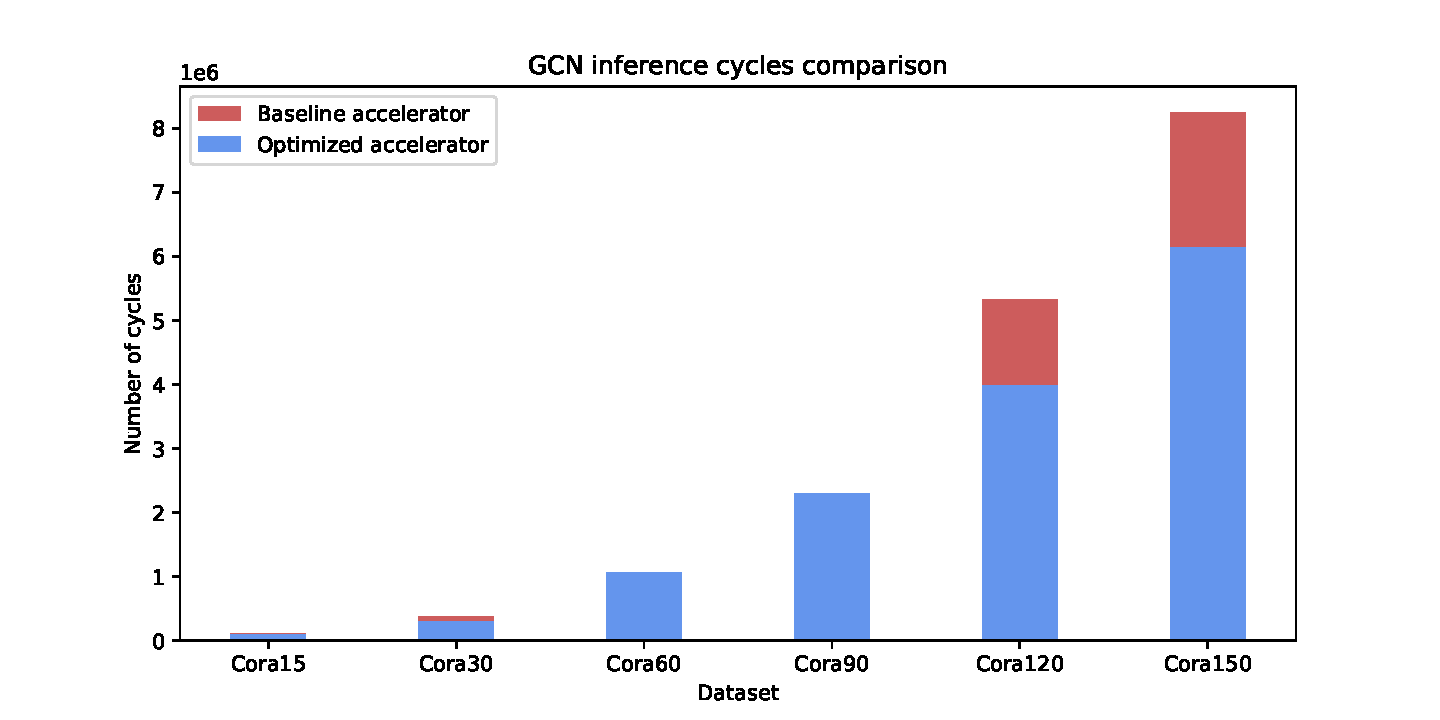
\includegraphics[height=0.4\textwidth]{Images/gcn_forward_cycles_comparison}
    \caption{GCN inference number of cycles comparison}
    \label{fig:gcn-inference-cycles-comparison}
\end{figure}

The results of this final evaluation are incredibly encouraging, showing significant improvement obtained by the optimized accelerator using two channels with on-chip BRAMs.
The speedup of the accelerator is still being affected by the size of the input matrices, but this was an expected result since the unrolling factor used is limited.
The accelerator's computational time is significantly lower with respect to the one measured on CPU with PyTorch, and for bigger dataset sizes the technique presented in Subsection~\ref{subsec:optimization-comparison} can be used, accelerating even more the computational performance of the accelerator.

The area of the accelerator, instead, is obviously affected by the sizes of the input matrices and of the unrolling factor.
This because more the matrices are big, more the parallel loop iterations will be and thus the parallel processing elements.

However, the possibilities offered by the proposed toolchain are various.
It is possible to use less memory channels with a lower loop unrolling factor to still have a big positive impact on performance, but limiting the accelerator area requirements.
Equation~\ref{eq:factor-relation} can be adapted also to this specific case, by considering the number of load and store and the size of the different loop iterations, becoming a valid indicator to decide which optimization to apply according to the dataset size.

\subsection{Model accuracy}
\label{subsec:modeol-accuracy}%

An evaluation of the model accuracy has been conducted for both the PyTorch-based implementation and the FPGA-accelerated version to ensure that the synthesis has no impact on accuracy.
Specifically, the process involved training the model in PyTorch, conducting inference to generate outputs, and saving all inputs and inference results in a binary file.
The binary file was then utilized to load all the data within a C file calling an external function, the forward kernel function, which was employed to run an RTL simulation of the FPGA accelerator using the same inputs as the PyTorch version.
The resulting inference output was saved and subjected to analysis, allowing for a comprehensive comparison with the PyTorch implementation.

\begin{table}[t]
\centering
    \begin{tabular}{|p{5em} c c c c|}
    \hline
%    \rowcolor{black!40}
    \textbf{Dataset} & \thead{PyTorch} & \thead{Accelerator} & \textbf{$\bm \epsilon$} & \thead{$\bm{\bar \epsilon}$} \T\B \\
    \hline \hline
    \textbf{Cora15} & 0.333 & 0.333 & 1.31E-06 & 0.26E-06 \T\B\\
    \hline
    \textbf{Cora30} & 0.333 & 0.333 & 8.64E-06 & 0.54E-06  \T\B\\
    \hline
    \textbf{Cora60} & 0.166 & 0.166 & 4.02E-06 & 0.25E-06 \T\B\\
    \hline
    \textbf{Cora90} & 0.555 & 0.555 & 19.47E-06 & 0.45E-06 \T\B\\
    \hline
    \textbf{Cora120} & 0.291 & 0.291 & 19.86E-06 & 0.27E-06 \T\B\\
    \hline
    \textbf{Cora150} & 0.533 & 0.533 & 23.84E-06 & 0.30E-06 \T\B\\
    \hline
    \end{tabular}
    \\[10pt]
    \caption[Model accuracy comparison between PyTorch and FPGA accelerator]{Model accuracy comparison between PyTorch and FPGA accelerator. $\epsilon$ = total error; $\bar \epsilon$ = average error.}
    \label{tab:model-accuracy-analysis}
\end{table}

Table~\ref{tab:model-accuracy-analysis} shows the accuracy of the PyTorch-based implementation and the FPGA accelerator.
Given that the datasets used are subsets of the Cora dataset and the small size of the training sets, the accuracy is understandably low.
In addition to assessing model accuracy, it also quantifies the overall value error, which is calculated as the cumulative difference between PyTorch and FPGA floating values, restricted to the inference output matrix cells associated with the test set.
Furthermore, the average floating error is determined by dividing the total error by the count of output matrix cells affected by the error.
The results indicate that the model accuracy has been maintained in the FPGA accelerator and that the average error does not increase as the dimension of the test set increases.
Nonetheless, the slight variation in the floating-point data precision between the PyTorch inference output and the FPGA accelerator, even with very low probability, may potentially cause an error in data classification, resulting in a difference of the accuracy, especially when dealing with very large datasets.

\section{Discussion}
\label{sec:sota-comparison}%

%The proposed design flow offers the flexibility of utilizing customized settings tailored to diverse applications, which presents a distinct advantage in contrast to the optimized pipeline offered by SODA-OPT~\cite{9786533}.
%The latter confines users to employ only the full unrolling optimization technique, which can represent a limitation when dealing with extensive loop iterations.
%This limitation prevents the fine-tuning of the balance between area utilization and performance, particularly when handling significant large loops, potentially leading to resource exhaustion and errors.
%In contrast, the design flow introduced in this thesis provides a more refined approach to customizing the trade-off between area and performance.
%It eliminates the need for mandatory double full unrolling when a single one is not sufficient, offering the flexibility to employ a partial unrolling factor.

The proposed design flow offers the flexibility of utilizing customized settings tailored to diverse applications.
Employing SODA-OPT~\cite{9786533} with its default optimized pipeline can result in excessive area consumption, which can lead to memory errors.
In contrast, this thesis provides a selection of SODA-OPT optimizations aimed at achieving improved performance, customizing the trade-off between area and performance.

A possible comparison involves FlowGNN~\cite{sarkar2022flowgnn}, which stands out among the state-of-the-art technologies introduced in Chapter~\ref{ch:chapter_three} as the only solution employing the HLS technique, which is also used in this thesis.
The toolchain proposed in this thesis, as well as the dataflow accelerator of FlowGNN, offers support for a diverse range of GNN models.
However, FlowGNN is limited to just four configurable parallelization parameters and focuses on delivering model-specific components, which limit the customization of the accelerator even further.
In contrast, the proposed toolchain offers many optimization passes from both SODA-OPT and PandA-Bambu, allowing users to finely customize and optimize the accelerator's capabilities.
Another significant advantage of the proposed toolchain is its ability to generate the accelerator directly from the PyTorch implementation, eliminating the need for low-level programming.
This sets it apart from FlowGNN, which offers pre-built models in C++.
The authors, through a small example, state that the provided models can be slightly changed to be adapted to different features.
However, to do this a minimum of experience with C++ is needed, and if the changes are substantial it could be a blocking factor.
On the contrary, the proposed toolchain, only requires knowledge in PyTorch, one of the most used the high-level framework for GNN implementations.

